% Options for packages loaded elsewhere
\PassOptionsToPackage{unicode}{hyperref}
\PassOptionsToPackage{hyphens}{url}
%
\documentclass[
]{article}
\usepackage{amsmath,amssymb}
\usepackage{lmodern}
\usepackage{iftex}
\ifPDFTeX
  \usepackage[T1]{fontenc}
  \usepackage[utf8]{inputenc}
  \usepackage{textcomp} % provide euro and other symbols
\else % if luatex or xetex
  \usepackage{unicode-math}
  \defaultfontfeatures{Scale=MatchLowercase}
  \defaultfontfeatures[\rmfamily]{Ligatures=TeX,Scale=1}
\fi
% Use upquote if available, for straight quotes in verbatim environments
\IfFileExists{upquote.sty}{\usepackage{upquote}}{}
\IfFileExists{microtype.sty}{% use microtype if available
  \usepackage[]{microtype}
  \UseMicrotypeSet[protrusion]{basicmath} % disable protrusion for tt fonts
}{}
\makeatletter
\@ifundefined{KOMAClassName}{% if non-KOMA class
  \IfFileExists{parskip.sty}{%
    \usepackage{parskip}
  }{% else
    \setlength{\parindent}{0pt}
    \setlength{\parskip}{6pt plus 2pt minus 1pt}}
}{% if KOMA class
  \KOMAoptions{parskip=half}}
\makeatother
\usepackage{xcolor}
\IfFileExists{xurl.sty}{\usepackage{xurl}}{} % add URL line breaks if available
\IfFileExists{bookmark.sty}{\usepackage{bookmark}}{\usepackage{hyperref}}
\hypersetup{
  pdftitle={Data \& Modeling section for Lab2},
  pdfauthor={Group 2: Jeremy Lan, Taehun Kim, Nicolas Loffreda},
  hidelinks,
  pdfcreator={LaTeX via pandoc}}
\urlstyle{same} % disable monospaced font for URLs
\usepackage[margin=1in]{geometry}
\usepackage{graphicx}
\makeatletter
\def\maxwidth{\ifdim\Gin@nat@width>\linewidth\linewidth\else\Gin@nat@width\fi}
\def\maxheight{\ifdim\Gin@nat@height>\textheight\textheight\else\Gin@nat@height\fi}
\makeatother
% Scale images if necessary, so that they will not overflow the page
% margins by default, and it is still possible to overwrite the defaults
% using explicit options in \includegraphics[width, height, ...]{}
\setkeys{Gin}{width=\maxwidth,height=\maxheight,keepaspectratio}
% Set default figure placement to htbp
\makeatletter
\def\fps@figure{htbp}
\makeatother
\setlength{\emergencystretch}{3em} % prevent overfull lines
\providecommand{\tightlist}{%
  \setlength{\itemsep}{0pt}\setlength{\parskip}{0pt}}
\setcounter{secnumdepth}{-\maxdimen} % remove section numbering
\usepackage{longtable} \usepackage{dcolumn}
\ifLuaTeX
  \usepackage{selnolig}  % disable illegal ligatures
\fi

\title{Data \& Modeling section for Lab2}
\author{Group 2: Jeremy Lan, Taehun Kim, Nicolas Loffreda}
\date{}

\begin{document}
\maketitle

\hypertarget{data}{%
\subsection{2. Data}\label{data}}

The dataset we will be using for this analysis is a subset of that
collected by Moro et al.~(2016). The dataset contains a representative
sample of 500 Facebook posts from a worldwide renowned cosmetic brand,
collected between January 1st and December 31st of 2014. By the time the
data was collected, Facebook was the most used social website, with
roughly 1.28 billion monthly active users (Insights 2014).

Each observation from the dataset represents a post from this company,
for which a variety of features have been collected.

Given the large sample size, we will use a randomized sub-sample of 150
observations for exploration purposes and the remaining 350 for running
the models. The only anomaly in the variables of interest is one missing
value for \texttt{paid} variable, which we will be removing from the
analysis, leaving us with a total of 499 observations.

\begin{center}
  Randomized sub-samples
\end{center}

\begin{center}
  \begin{tabular}{l r}
    \hline
    Split     &  \\
    \hline
    Exploration & 150 \\
    Test        & 349             \\
    \hline
    Total       & 499             \\
    \hline
  \end{tabular}
\end{center}

\hypertarget{engaged-users}{%
\subsubsection{2.1 Engaged users}\label{engaged-users}}

The outcome variable will be the number of unique \emph{engaged users}
the post had through its lifetime. An engaged user is defined as someone
who clicked in the post. Looking into this variable, we can see that it
is fairly skewed to the right. To make the variable easier to work with,
we will be applying a log transformation:

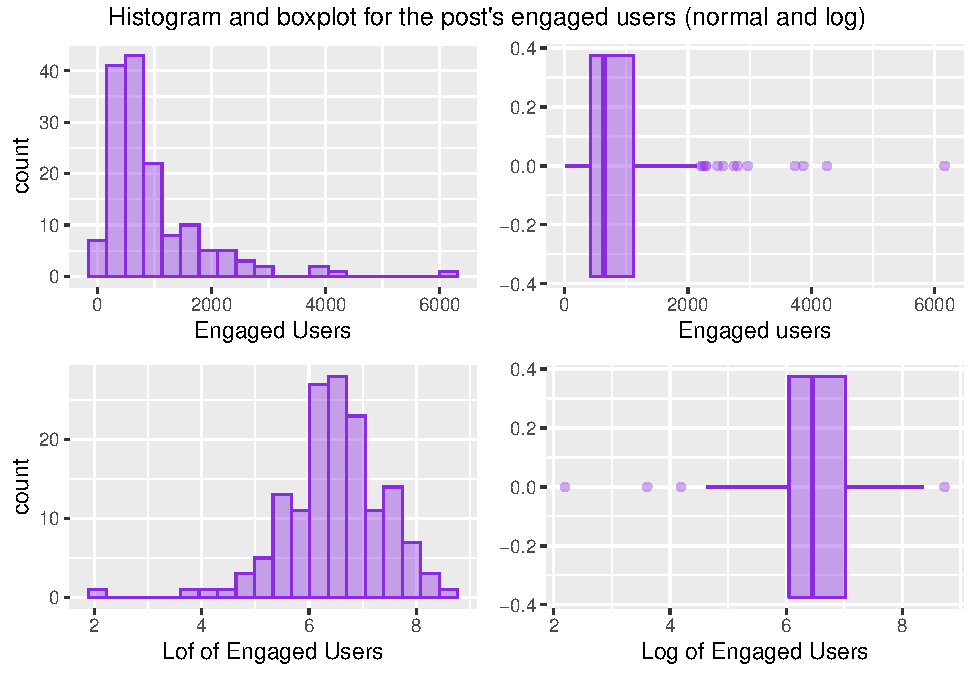
\includegraphics{lab2_datasplit_noba_nico_files/figure-latex/unnamed-chunk-2-1.pdf}

\hypertarget{category-and-type}{%
\subsubsection{2.2 Category and Type}\label{category-and-type}}

The main variables we want to measure the impact on engaged users are
the \texttt{type} and \texttt{category} of the post. The \texttt{type}
is categorized in Photo, Video, Link or Status, and it represents what
kind of content the post contained. We can see that most of the posts
published were photos:

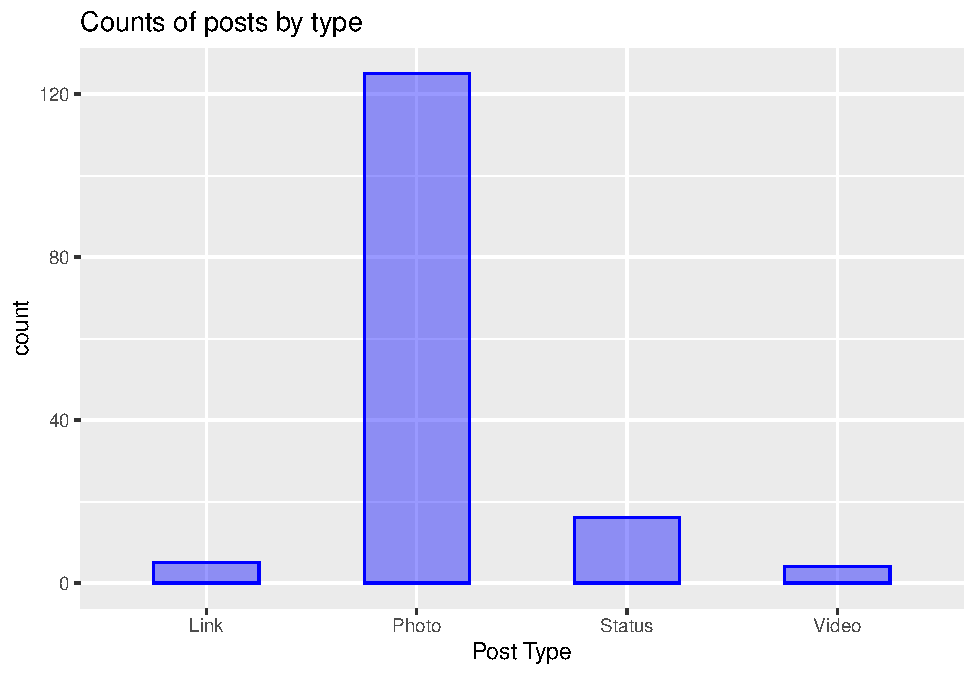
\includegraphics{lab2_datasplit_noba_nico_files/figure-latex/unnamed-chunk-3-1.pdf}

On the other hand, the category describes how the content of the post
was displayed to the user. There were 3 distinct categories the dataset
differentiates: - Action: Special offers and contests - Product: Direct
advertisement or explicit brand content - Inspiration: Non-explicit
brand related content

The number of posts published of each category are as follows:

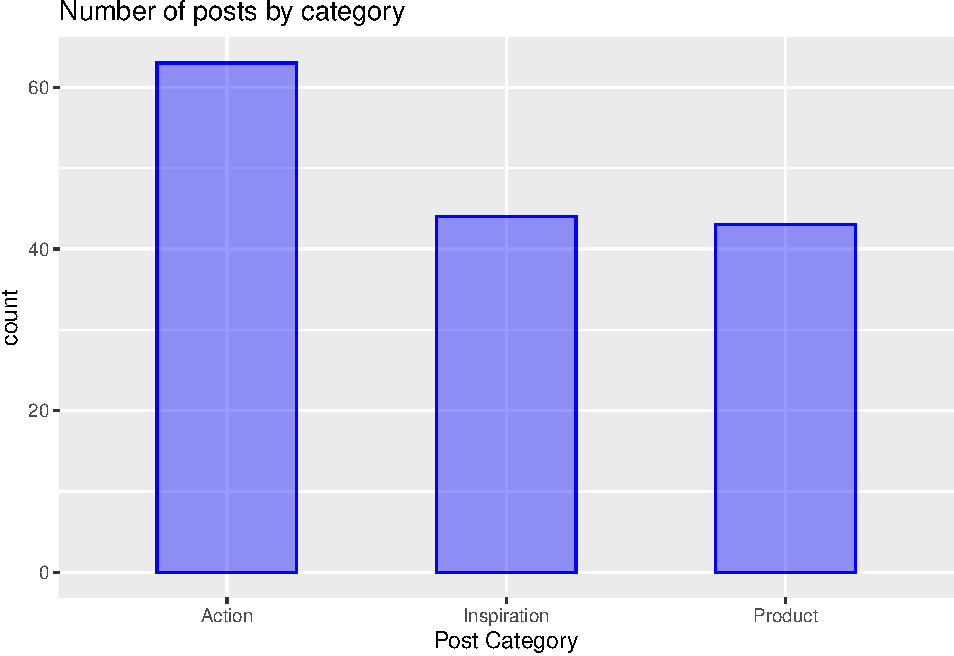
\includegraphics{lab2_datasplit_noba_nico_files/figure-latex/unnamed-chunk-4-1.pdf}

\hypertarget{covariates}{%
\subsubsection{2.3 Covariates}\label{covariates}}

\hypertarget{paid}{%
\paragraph{2.3.1 Paid}\label{paid}}

Among the covariates we will be including in the model is paid
advertising. The variable \texttt{paid} will be encoded as a dummy
variable to indicate whether the post had any paid media associated with
it or not. We can see that in the exploratory dataset,
\textasciitilde32\% of all the posts had some kind of paid media
support:

\begin{center}
  Paid media support
\end{center}

\begin{center}
  \begin{tabular}{l r}
    \hline
    Media Support   & Number of posts \\
    \hline
    No Paid support & 114             \\
    Paid support    & 36             \\
    \hline
    Total           & 150             \\
    \hline
  \end{tabular}
\end{center}

\hypertarget{period-of-day-and-day-of-the-week}{%
\paragraph{2.3.2 Period of day and Day of the
week}\label{period-of-day-and-day-of-the-week}}

The last variables we will be including as control are the period of the
day and the day of the week the post was published to account for the
differences that may exist on user activity at different times and days.

In particular, we will distinguish 4 periods of the day, overnight,
morning, afternoon and evening. The first going from 12am to 6am, the
second one from 6am to 12pm, then 12pm to 6pm, and 6pm to 12am.

On the other hand, the days of the week will be divided into weekdays
and weekends. This will be encoded in a dummy set to 1 if the period is
a weekend.

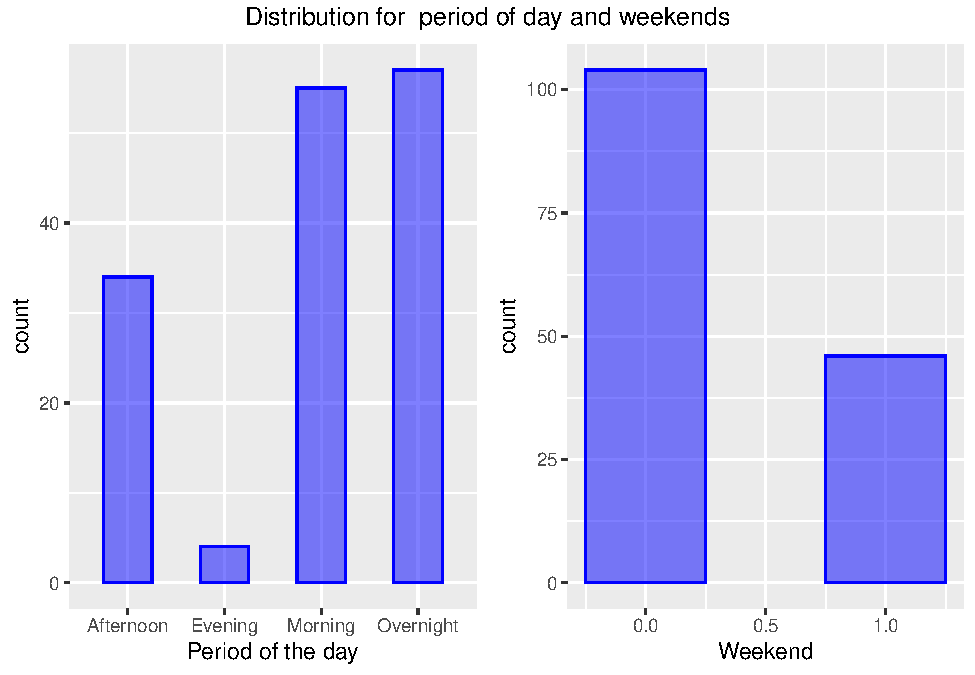
\includegraphics{lab2_datasplit_noba_nico_files/figure-latex/unnamed-chunk-5-1.pdf}

\hypertarget{model}{%
\subsection{3. Model}\label{model}}

\hypertarget{base-model}{%
\subsubsection{3.1 Base Model}\label{base-model}}

As explained in the data section, we will be applying a log
transformation to the outcome variable, engaged users. The base model
will only include type and category as main explanatory variables:

\(\widehat{\log(engaged\_users)}=\beta_0 + \beta_1 \text{ } type + \beta_2 \text{ } category\)

\hypertarget{adding-covariates}{%
\subsubsection{3.2 Adding Covariates}\label{adding-covariates}}

With the base model established, we will be including as control
variables paid media efforts, brand awareness, day of the week and
period of the day. All these as described on the data section:

\begin{align*}
\widehat{\log(engaged\_users)}=\beta_0 &+ \beta_1 \text{ } type + \beta_2 \text{ } category\\ 
&+ \beta_3 \text{ } paid +\beta_4 \text{ } day\_of\_week + \beta_5 \text{ } period\_of\_day
\end{align*}

\hypertarget{adding-interaction-term}{%
\subsubsection{3.3 Adding Interaction
term}\label{adding-interaction-term}}

As a next model, we will be including an interaction term to account to
see how the different types behave when paired with the different
categories:

\begin{align*}
\widehat{\log(engaged\_users)}=\beta_0 &+ \beta_1 \text{ } type + \beta_2 \text{ } category + \beta_3 \text{ } paid \\
& + \beta_4 \text{ } day\_of\_week + \beta_5 \text{ } period\_of\_day + \beta_6 \text{ } type*category
\end{align*}

\hypertarget{standard-errors}{%
\subsubsection{3.4 Standard Errors}\label{standard-errors}}

We understand that certain dependencies may exist among the posts given
that they are all from the same company. This means that the people that
know the brand and interact with the social site and posts may be
similar on the different posts.

Because of this reason, we will be using \emph{robust clustered standard
errors} to adjust the significance for any independence that may exist.

\hypertarget{results}{%
\subsection{4. Results}\label{results}}

Results of the models described are shown in the table below:

\begin{longtable}{@{\extracolsep{5pt}}lccc}
  \caption{} 
  \label{} 

\\[-1.8ex]\hline 
\hline \\[-1.8ex] 
 & \multicolumn{3}{c}{\textit{Dependent variable:}} \\ 
\cline{2-4} 
\\[-1.8ex] & \multicolumn{3}{c}{log(Engaged Users)} \\ 
\\[-1.8ex] & (1) & (2) & (3)\\ 
\hline \\[-1.8ex] 
 Type - Photo & 0.944$^{***}$ & 0.939$^{***}$ & 0.951$^{***}$ \\ 
  & (0.259) & (0.273) & (0.292) \\ 
  & & & \\ 
 Type - Status & 1.822$^{***}$ & 1.883$^{***}$ & 2.330$^{***}$ \\ 
  & (0.329) & (0.346) & (0.504) \\ 
  & & & \\ 
 Type - Video & 1.696$^{***}$ & 1.594$^{***}$ & 1.609$^{***}$ \\ 
  & (0.441) & (0.367) & (0.381) \\ 
  & & & \\ 
 Category - Inspiration & 0.139 & 0.094 & 0.335 \\ 
  & (0.101) & (0.102) & (0.289) \\ 
  & & & \\ 
 Category - Product & $-$0.007 & $-$0.001 & $-$0.387 \\ 
  & (0.119) & (0.122) & (0.469) \\ 
  & & & \\ 
 Paid Media &  & 0.236$^{**}$ & 0.226$^{**}$ \\ 
  &  & (0.093) & (0.094) \\ 
  & & & \\ 
 Period - Evening &  & $-$0.362 & $-$0.359 \\ 
  &  & (0.490) & (0.488) \\ 
  & & & \\ 
 Period - Morning &  & $-$0.340$^{***}$ & $-$0.334$^{***}$ \\ 
  &  & (0.116) & (0.116) \\ 
  & & & \\ 
 Period - Overnight &  & $-$0.129 & $-$0.123 \\ 
  &  & (0.117) & (0.116) \\ 
  & & & \\ 
 Weekend &  & $-$0.156 & $-$0.166$^{*}$ \\ 
  &  & (0.100) & (0.100) \\ 
  & & & \\ 
 Interaction - Photo:Inspiration &  &  & $-$0.219 \\ 
  &  &  & (0.303) \\ 
  & & & \\ 
 Interaction - Status:Inspiration &  &  & $-$1.678 \\ 
  &  &  & (1.259) \\ 
  & & & \\ 
 Interaction - Video:Inspiration &  &  &  \\ 
  &  &  &  \\ 
  & & & \\ 
 Interaction - Photo:Product &  &  & 0.371 \\ 
  &  &  & (0.480) \\ 
  & & & \\ 
 Interaction - Status:Product &  &  &  \\ 
  &  &  &  \\ 
  & & & \\ 
 Interaction - Video:Product &  &  &  \\ 
  &  &  &  \\ 
  & & & \\ 
 Constant & 5.431$^{***}$ & 5.611$^{***}$ & 5.596$^{***}$ \\ 
  & (0.249) & (0.292) & (0.307) \\ 
  & & & \\ 
\hline \\[-1.8ex] 
Observations & 349 & 349 & 349 \\ 
R$^{2}$ & 0.147 & 0.193 & 0.203 \\ 
Adjusted R$^{2}$ & 0.135 & 0.169 & 0.172 \\ 
Residual Std. Error & 0.815 (df = 343) & 0.798 (df = 338) & 0.797 (df = 335) \\ 
\hline 
\hline \\[-1.8ex] 
\textit{Note:}  & \multicolumn{3}{r}{$^{*}$p$<$0.1; $^{**}$p$<$0.05; $^{***}$p$<$0.01} \\ 
\end{longtable}

All the different types of posts are significant to an \(\alpha\) level
of 0.05 across all models, with Link being the omitted type. From the
magnitude of the coefficients we can see that Video, Status and Photo
perform much better than Link, with Status yielding the highest increase
on engaged users. All these coefficients are quite stable across models
as well. As for the categories, none of them are significant which is
quite surprising.

The second model includes the covariates paid, period of the day and
weekday. The results are similar to those of the base model. As
expected, we see that paid comes as significant with a positive
coefficient, although smaller in magnitude than any of the post types.
Posting on weekends doesn't seem to be significant in any of the models
but some of the periods do. With the omitted day period being the
afternoon, we see that morning is highly significant and has a negative
coefficient. This implies that the period of the day associated with
higher engagement is the afternoon.

We ran a Wald Test between the base and the covariate models and it
yields a low p-value, meaning that some of the covariates are helping to
explain the variability of the engaged users. This phenomenon can also
be appreciated in the coefficient of determination (i.e.~\(R^2\)), as it
jumps from 14\% in the first model, to 17\% after the addition of these
covariates.

\begin{verbatim}
## Wald test
## 
## Model 1: log(lifetime_engaged_users) ~ 1 + type + category_str
## Model 2: log(lifetime_engaged_users) ~ 1 + type + category_str + paid + 
##     period_of_day + weekend
##   Res.Df Df     F   Pr(>F)   
## 1    343                     
## 2    338  5 4.191 0.001042 **
## ---
## Signif. codes:  0 '***' 0.001 '**' 0.01 '*' 0.05 '.' 0.1 ' ' 1
\end{verbatim}

When looking at the model with the interaction term and covariates, we
see similar results than the previous one, but with a few modifications.
The first thing we see is that now posting on weekends is significant to
an \(\alpha\) level of 0.1. We also see that the coefficient is
negative, implying that posting during weekdays is associated with more
engaged users.

Examining the interaction term, we notice that none of the terms are
significant, which is quite surprising. Some of the coefficients are
missing, implying high correlation between them.

Last, we examine the Wald Test between the model with covariates and the
interaction model, and the high p-value indicates that the interaction
term doesn't add explanatory power to the model. This can also be
appreciated by the fact that the \(R^2\) doesn't increase significantly
from one model to another.

\begin{verbatim}
## Wald test
## 
## Model 1: log(lifetime_engaged_users) ~ 1 + type + category_str + paid + 
##     period_of_day + weekend
## Model 2: log(lifetime_engaged_users) ~ 1 + type * category_str + paid + 
##     period_of_day + weekend
##   Res.Df Df      F Pr(>F)
## 1    338                 
## 2    335  3 0.7353 0.5316
\end{verbatim}

\end{document}
